\section{Incremental Approach}
\label{Section:IncrementalApproach}

In multi-layer QAOA, increasing the number of layers also increases the number of parameters
to be optimized. Finding global optima is considerably simpler for $p=1$ (i.e., two parameters)
than for circuits with many layers. Moreover, when a new layer is added, the previously optimized
solution remains valid within the enlarged parameter space: the parameters corresponding to the
first $p$ layers can be initialized with their previously optimized values, while the newly
introduced parameters can be set to zero. Consequently, adding an additional layer
($p \rightarrow p+1$) can only maintain or improve performance relative to the previous iteration.

This observation motivates a progressive training strategy, often referred to as an \emph{incremental}
approach, which proceeds as follows:
\begin{enumerate}
    \item Analyze the cost function landscape for $p=1$ to select initial parameters 
    $\gamma_1$ and $\beta_1$ close to the optimal region (Fig.~\ref{fig:costfun_landscape}).
    \item Optimize QAOA with $p=1$ to obtain the parameters 
    $\widetilde{\gamma}_1$ and $\widetilde{\beta}_1$.
    \item Optimize QAOA with $p=2$, initializing 
    $\gamma_1=\widetilde{\gamma}_1$ and $\beta_1=\widetilde{\beta}_1$, 
    and selecting suitable initial values for $\gamma_2$ and $\beta_2$ using an appropriate
    heuristic (Sec.~\ref{Section:ParameterInitialization}). This yields the updated parameters 
    $\widetilde{\gamma}_1, \widetilde{\gamma}_2, \widetilde{\beta}_1, \widetilde{\beta}_2$.
    \item Repeat this procedure iteratively up to the desired depth $p$, each time initializing
    with the optimized parameters from the previous iteration and applying a strategy to set
    the new layer's parameters.
\end{enumerate}

\begin{figure}[h]
    \centering
    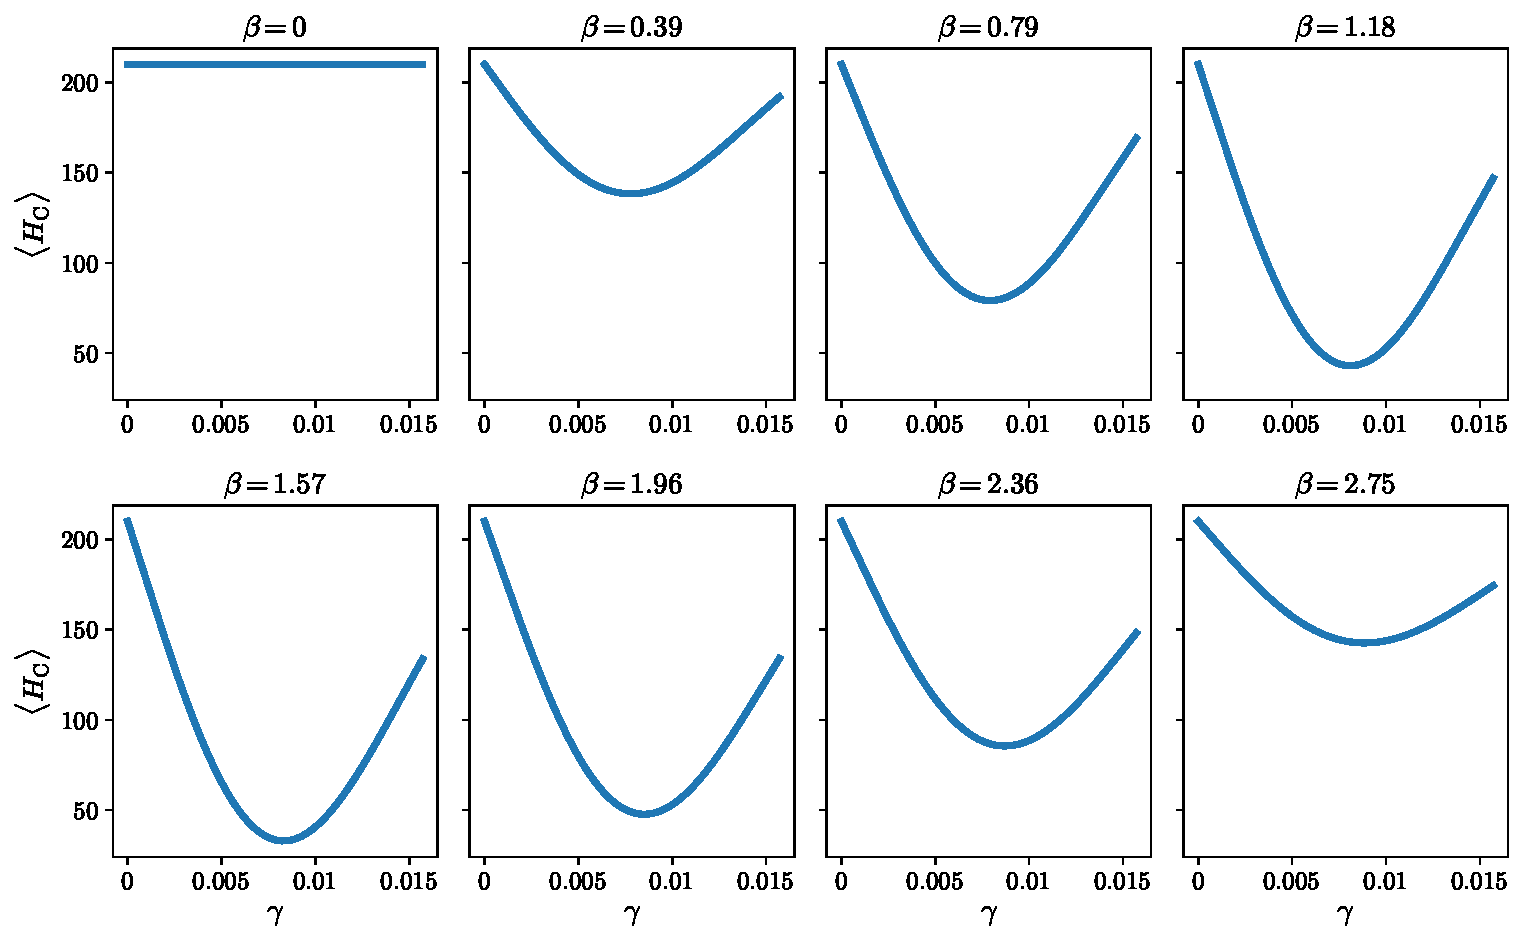
\includegraphics[width=1\textwidth]{03-methodology/figs/costfun_landscape.pdf}
    \caption{Cost function profile for the quadratic Hamiltonian when $N=21$. After this
    analysis, $\gamma_0=0.0075$ and $\beta_0=1.57$ are used as initial parameters for $p=1$.
    Maximum $\gamma$ is determined as the value that causes angle folding for the
    maximum energy eigenvalue, i.e. $e^{-i \gamma_\mathrm{max} E_\mathrm{max}} = e^{-2\pi i}$.}
    \label{fig:costfun_landscape}
\end{figure}